\chapter[Foundations of Open-World Agent--Environment Interaction]{Foundations of Open-World Agent--Environment Interaction\footnotemark}
\label{ch:foundations}
\footnotetext{Portions of this chapter are based on: S.~Goel, P.~Lymperopoulos, R.~Thielstrom, E.~Krause, P.~Feeney, P.~Lorang, S.~Schneider, Y.~Wei, E.~Kildebeck, S.~Goss, M.~C.~Hughes, L.~Liu, J.~Sinapov, and M.~Scheutz, ``A Neurosymbolic Cognitive Architecture Framework for Handling Novelties in Open Worlds,'' \textit{Artificial Intelligence}, vol.~331, p.~104111, 2024.}

This chapter develops the formal and conceptual foundations that support the remainder of the dissertation. 
We begin by defining the open-world setting: environments in which an agent's knowledge is necessarily incomplete with respect to the true state of the world
%  and where this incompleteness can change over time in ways that were not anticipated during agent's design
  (\cref{sec:open_world_environments}). We then formalize the concept of novelty as a mismatch between an agent's internal models and the environment---and introduce a taxonomy that classifies novelties by their impact on task performance (\cref{sec:novelty}). With the setting and the problem defined, we turn to the agent itself: how it represents, reasons about, and acts upon the world, integrating symbolic planning and subsymbolic execution into a unified decision-making framework (\cref{sec:agent_framework}). Finally, we examine the role of structured abstractions in mediating the agent--environment interaction, arguing that the choice of abstraction determines whether novelty-induced mismatch can be handled through efficient adaptation and generalizable behavior (\cref{sec:abstractions}).

Together, these foundations establish the formal vocabulary and conceptual claims that the subsequent chapters build upon: benchmark environments for evaluating agents under controlled novelty (\cref{ch:benchmarks}), action abstractions that enable efficient adaptation under failure (\cref{ch:rapid_learn}), and interaction abstractions that support generalization across objects and embodiments (\cref{ch:generalization}).

\section{Open-World Environments}
\label{sec:open_world_environments}

Autonomous agents operate within environments that they must perceive, reason about, and act upon in order to achieve their goals. In this section, we formalize the structure of such environments and the agents that inhabit them, and distinguish between the closed-world settings that underlie most current AI research and the open-world settings that motivate this dissertation.

\subsection{The Environment}
\label{sec:environment}

We consider a task environment $\Env = \langle \EnvStates, \EnvDynamics \rangle$ consisting of a set of environment states $\EnvStates$ and a set of dynamics $\EnvDynamics$ that govern how states evolve over time. The environment may contain any number of objects and other agents as part of its state, and its dynamics may be deterministic or stochastic. Environment states are agent-independent in the sense that they specify the underlying configuration of the world whether or not any particular agent observes or represents them correctly.

At any given time $t$, the environment is in some state $e_t \in \EnvStates$. The dynamics $\EnvDynamics$ define how this state changes, both due to the natural evolution of the environment and as a consequence of actions taken by agents within it. In general, an agent does not have direct access to the full environment state $e_t$; instead, it observes the environment through its sensors and acts upon it through its effectors, as described below.

\subsection{The Agent}
\label{sec:agent}

An agent $\Agent = \langle \Sensors, \Effectors, \KnowledgeRepo, \vdash \rangle$ is defined by four components: a set of sensors $\Sensors$ that allow it to perceive the environment, a set of effectors $\Effectors$ that allow it to act upon it, a knowledge repository $\KnowledgeRepo$ that stores what the agent knows about the world, and an inference mechanism $\vdash$ that enables the agent to reason over its knowledge.

The knowledge repository $\KnowledgeRepo = (\KB, \SubsymbolicKB)$ is composed of two complementary parts. The knowledge base $\KB$ stores explicit symbolic knowledge---facts, rules, and relational descriptions expressed in a formal language $\Language$. The subsymbolic component $\SubsymbolicKB$ stores knowledge in distributed representations, such as the weights of neural networks that encode policies, value functions, or perceptual models. The inference mechanism $\vdash$ operates over both components: for $\KB$, it may take the form of logical deduction or planning; for $\SubsymbolicKB$, it corresponds to forward inference through learned models.

At time $t$, the agent's sensors generate internal representations of the partially observed environment state. Based on these observations and its knowledge $\KnowledgeRepo$, the agent selects actions through its inference mechanism and executes them via its effectors, producing changes in the environment state. This perceive--reason--act cycle defines the agent's ongoing interaction with the world.

\subsection{Closed-World and Open-World Assumptions}
\label{sec:closed_open}

The distinction between closed-world and open-world settings concerns the relationship between the agent's knowledge and the environment.

Under closed-world assumptions, the agent's representational vocabulary and task model are treated as fixed and sufficient for the situations the agent may encounter. Specifically, the relevant objects, predicates, observations, actions, rewards, dynamics, and action effects are assumed to fall within the agent's predefined modeling framework. This assumption has been productive: it underlies classical planning \citep{fikes1971strips, mcdermott1998pddl}, standard reinforcement learning formulations \citep{sutton2018reinforcement}, and many supervised learning approaches to perception. Under these assumptions, the primary challenge is computational---finding good plans, learning effective policies, or achieving accurate classification within a fixed representational space.

In open-world environments, this assumption is violated. The environment may contain objects, dynamics, or relationships that the agent's models do not represent. New objects may appear that do not correspond to any known category. Actions may produce effects that differ from what the agent's models predict. Task structure may change in ways that invalidate previously successful strategies. Critically, these changes need not be adversarial or extreme: even routine variation in everyday environments can fall outside the scope of models designed under closed-world assumptions.

This gap between the agent's knowledge and the true state of the world is not merely a quantitative shortcoming that can be addressed by training on more data or enumerating more states. It is a qualitative property of the agent--environment relationship: the world may contain structure that is not derivable from, or even expressible within, the agent's current representational framework. This observation motivates the formal treatment of novelty developed in the next section.

\subsection{A Running Example: The Crafting Agent}
\label{sec:running_example}

To make the framework concrete, we introduce a running example that will be used throughout this chapter and the remainder of the dissertation. Consider an agent operating in a gridworld environment inspired by the crafting mechanics of Minecraft. The environment contains objects such as trees, crafting tables, ores, and storage containers. The agent can perform actions such as navigating to objects, breaking trees to obtain logs, crafting logs into planks and sticks, and assembling complex items using crafting recipes. The agent's task is to craft a target item---say, a pogostick---which requires collecting and combining resources in a specific sequence.

In this setting, the agent maintains symbolic knowledge of the objects in the environment, their properties, the available crafting recipes, and the operators it can use (e.g., \texttt{break\_tree}, \texttt{craft\_planks}, \texttt{craft\_pogostick}). Each operator is associated with an executor---a policy that carries out the corresponding action in the environment. The agent generates a plan (a sequence of operators) and executes it step by step. Under closed-world conditions, where the environment matches the agent's models, this process succeeds reliably.

Now suppose the environment changes while the agent is performing its task. A new entity---a supplier---appears and may affect the agent's ability to obtain resources. Or the properties of a known object change: trees become unbreakable unless the agent first acquires a new tool, an axe. Or a crafting recipe is altered so that a previously unnecessary ingredient is now required. Each of these changes may constitute a novelty for the agent: an aspect of the environment that is not derivable from, or not expressible within, its current knowledge repository. How the agent responds---whether it can detect the change, diagnose its impact, and adapt its behavior---depends on the structure of its representations and reasoning capabilities. The formal treatment of novelty in \cref{sec:novelty} and the agent framework in \cref{sec:agent_framework} provide the machinery for analyzing these situations precisely.

\begin{figure}[t]
\centering
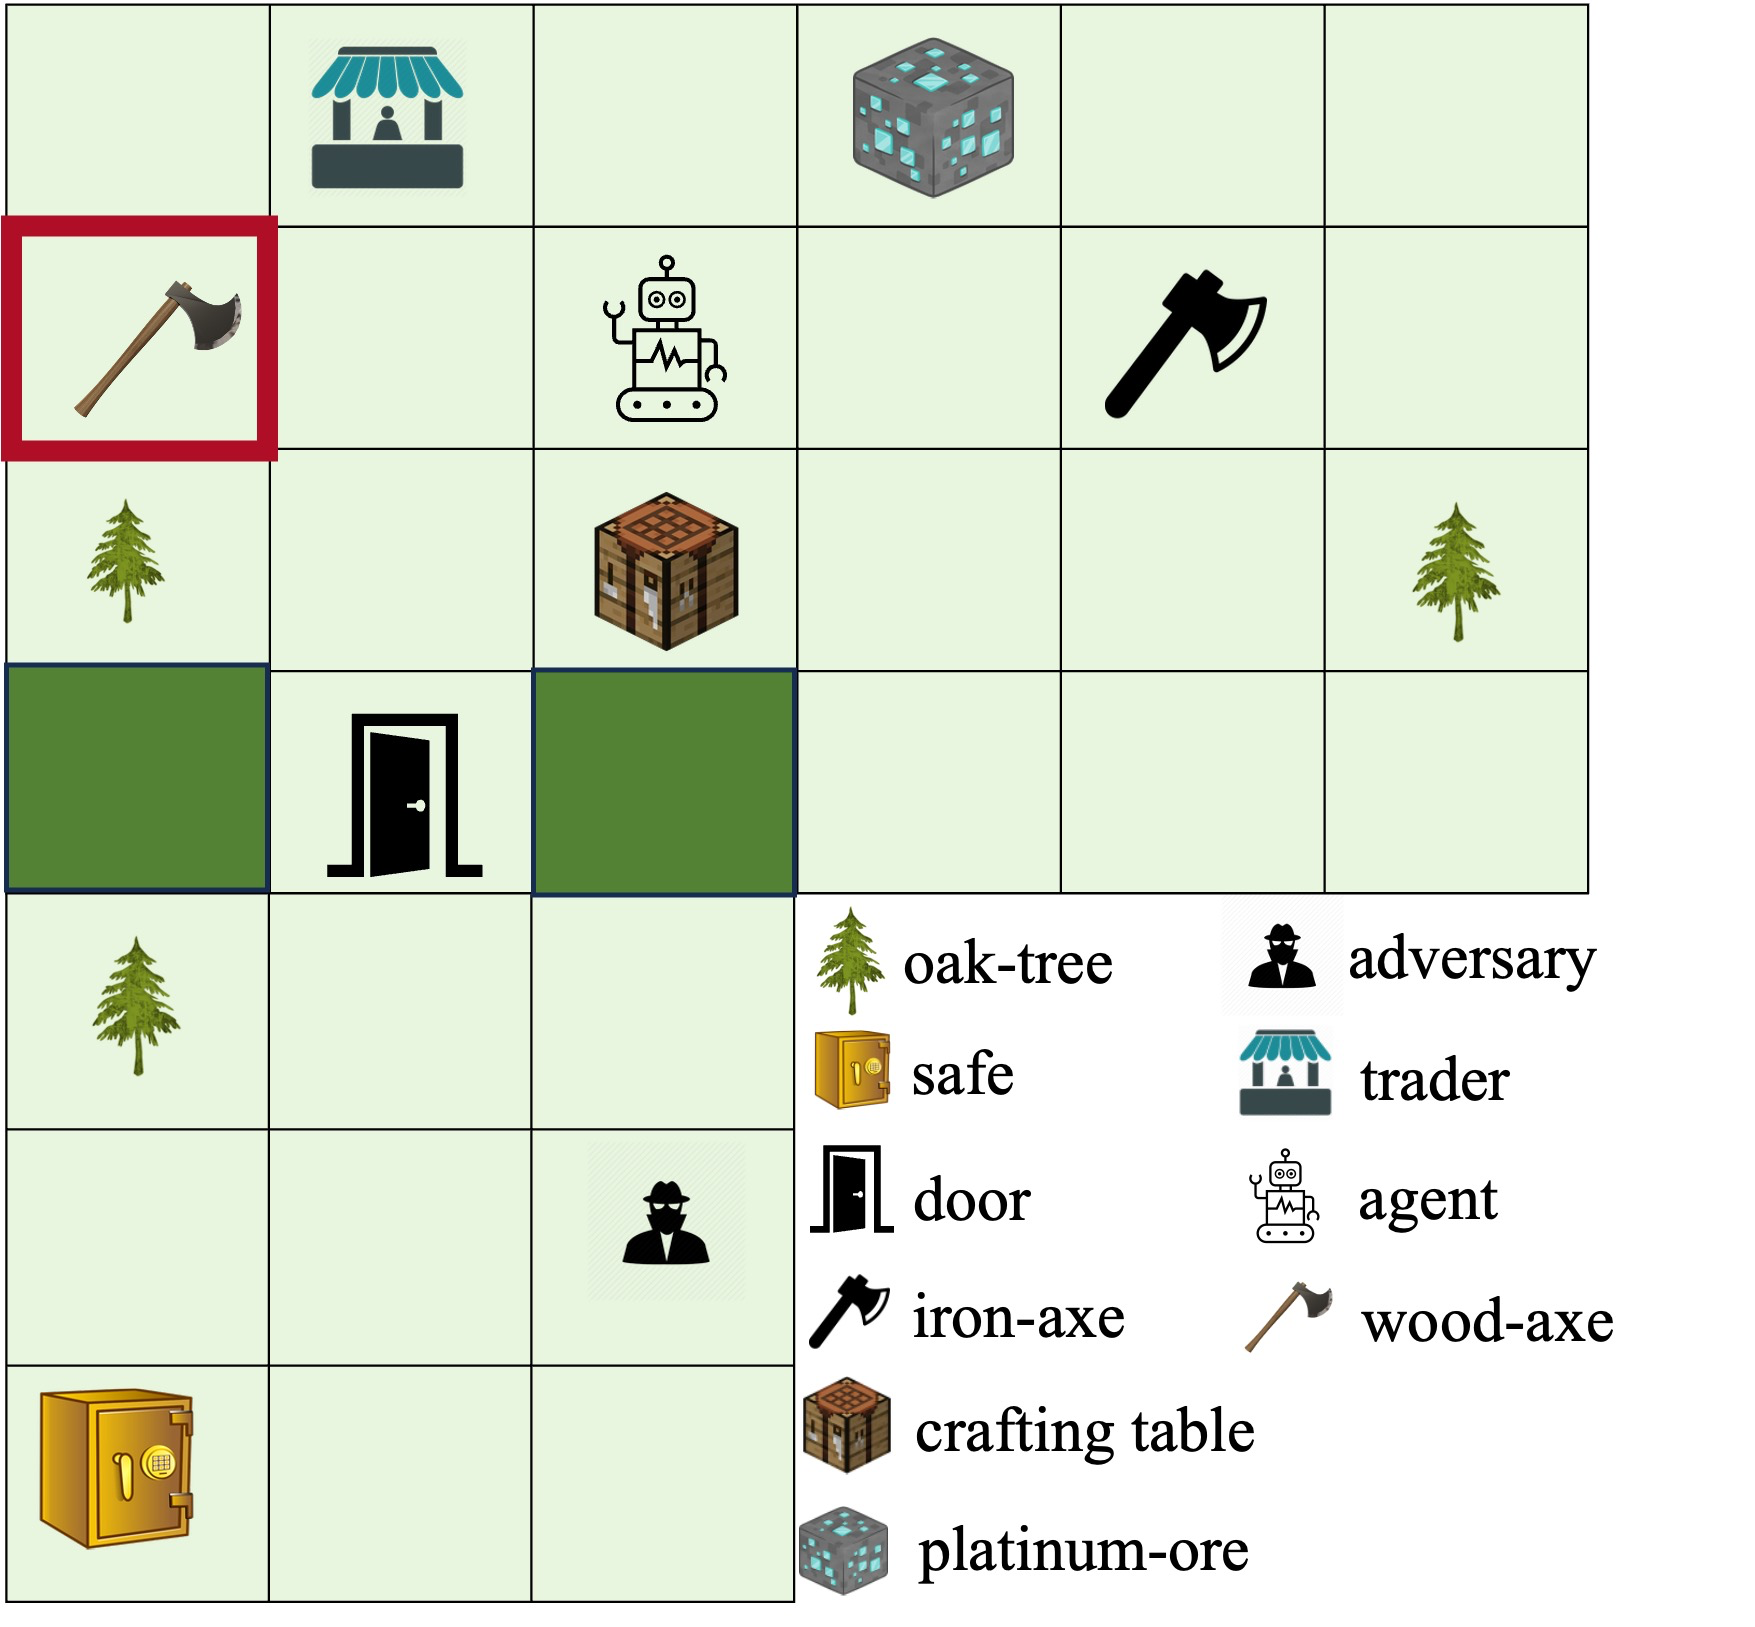
\includegraphics[width=0.6\textwidth]{figures/chapter2/Picture1_with_novelty.png}
\caption[The crafting gridworld environment]{The crafting gridworld environment used as a running example throughout this dissertation. The agent (center) operates among objects such as trees, crafting tables, and ores. A novel actor---the supplier, highlighted in blue---has been introduced and may affect the agent's ability to complete its task. Adapted from \citet{goel2024neurosymbolic}.}
\label{fig:gridworld}
\end{figure}

\subsection{Environment States and Agent Representations}
\label{sec:state_representations}

% The distinction between what exists in the environment and what the agent can represent is central to the framework.
 An environment state $e \in \EnvStates$ specifies the complete configuration of the world at a given time, including all objects, their properties, spatial arrangements, and dynamic relationships. The agent, however, does not operate over environment states directly. Instead, it constructs representations of the world using its available representational resources.

At the symbolic level, the agent uses a formal language $\Language$, consisting of predicates, variables, constants, and possibly functions, to describe aspects of the environment. A symbolic state description $\SymState \in \SymStates$ is a partial description of an environment state in this language. In planning domains, this description can be instantiated as a set of fluents $\Fluents$---state variables whose values may change over time---or as a set of grounded predicates that are used by the planner. When unlisted predicates are treated as false, this is a closed-world convention of the planning representation rather than a claim that the agent has complete knowledge of the environment.

At the subsymbolic level, the agent may represent the environment through continuous state vectors $s \in \States$, which may include raw sensory observations (e.g., images, Virtual LiDAR representations), learned feature representations, or structured numerical descriptions of the environment. These representations are typically used for perception and low-level control, and may be learned from data rather than explicitly defined. The agent's knowledge repository $\KnowledgeRepo$ contains the symbolic and subsymbolic representations that it uses to reason about the world and select actions. The inference mechanism $\vdash$ operates over these representations to generate plans, predict outcomes, and select actions. The agent's sensors and effectors mediate the mapping between the environment and its internal representations, but this mapping is not necessarily complete or accurate.

% An important consequence of this framework is that the mapping between environment states and agent representations is not one-to-one. Multiple environment states may be indistinguishable under the agent's current representational capacity, and a single environment state may be represented differently at different levels of abstraction. This gap between environment states and agent representations creates the space in which novelty can arise: aspects of the environment may exist, affect task performance, and yet not be derivable or representable within the agent's current knowledge repository.

% Content moved to chapters/chapter4_preliminaries/novelty.tex
% (formal novelty definition and taxonomies now live in Chapter 4).
% This file is retained only so old paths do not silently disappear from git history reviews.


\section{A Framework for Open-World Agents}
\label{sec:agent_framework}

Having defined the environment and the nature of novelty, we now turn to the structure of the agent itself. The agents studied in this dissertation operate by combining symbolic reasoning at the level of task planning with subsymbolic execution at the level of environment interaction and execution. 
This section formalizes the components of this framework: symbolic planning, reinforcement learning, and their integration into a hybrid architecture. More specifically, we will provide the preliminary definitions of the components of the agent that will be used throughout the dissertation.
% Rather than presenting these as independent formalisms, we develop them as complementary components of a single agent that must reason, act, and adapt under novelty.

\subsection{Symbolic Planning}
\label{sec:symbolic_planning}

The agent's high-level decision-making is conducted through symbolic planning, which enables structured reasoning over abstract representations of states and actions. Following the representation introduced in \cref{sec:state_representations}, we adopt a STRIPS-style formalism \citep{fikes1971strips} in which symbolic states, preconditions, and effects are defined over grounded literals. This representation is used throughout the dissertation and provides the foundation for the operator--executor consistency conditions developed in \cref{ch:rapid_learn}.

\paragraph{Symbolic states.}
Let $\Language$ be the agent's formal language of predicates, variables, constants, and possibly functions. A \emph{grounded literal} is an atom $p(c_1, \ldots, c_k)$ or its negation $\neg p(c_1, \ldots, c_k)$, where $p$ is a predicate symbol and each $c_i$ is a constant. We write $\Lit$ for the set of all grounded literals over $\Language$. A symbolic state $\SymState \in \SymStates$ is a consistent subset $\SymState \subseteq \Lit$ containing no atom together with its negation. Under the closed-world convention (\cref{sec:state_representations}), literals not contained in $\SymState$ are treated as false. In propositional planning domains, $\SymState$ is typically represented by the set of positive ground atoms that hold; negated literals are implicit. A conjunction of positive literals $\Phi$ is satisfied in $\SymState$, written $\SymState \models \Phi$, if and only if $\Phi \subseteq \SymState$.

\paragraph{Planning domain and task.}
The agent's symbolic model is organized into a \emph{planning domain} and a \emph{planning task}. The planning domain $\PlanningDomain = \langle \Fluents, \Operators \rangle$ specifies the domain vocabulary: $\Fluents$ is the set of fluent symbols (predicate and function symbols whose grounded instances may change over time), and $\Operators$ is a set of operator schemas. A planning task is a tuple $\PlanningTask = \langle \PlanningDomain, \SymState_0, \Goal \rangle$, equivalently written $\PlanningTask = \langle \Fluents, \Operators, \SymState_0, \Goal \rangle$, where $\SymState_0 \in \SymStates$ is the initial state and $\Goal$ is a goal condition over literals (a conjunction of positive literals, or a disjunctive normal form thereof). Throughout the dissertation, we write $\Pre_\Operator = \psi_\Operator$ for the precondition literal set of operator $\Operator$ and $\Eff_\Operator = \omega_\Operator$ for its effect literal set.

\paragraph{Operators.}
Each operator schema defines a parameterized action template. A \emph{grounded operator} $\Operator \in \Operators$ is specified as
\[
\Operator = \langle \Pre_\Operator, \Eff_\Operator^+, \Eff_\Operator^- \rangle,
\]
where $\Pre_\Operator \subseteq \Lit$ is a set of positive literals whose conjunction must hold for the operator to be applicable, $\Eff_\Operator^+ \subseteq \Lit$ is the \emph{add list} of positive literals made true by the operator, and $\Eff_\Operator^- \subseteq \Lit$ is the \emph{delete list} of positive literals made false. When an operator's effects are referenced as a single set---for example, in effect satisfaction checks during execution---$\Eff_\Operator$ denotes the postcondition add list $\Eff_\Operator^+$. Operator schemas are instantiated over domain objects to produce grounded operators; for instance, a schema \texttt{break(?x)} grounded with a tree constant yields a grounded operator with concrete preconditions and effects. Domains with numeric fluents extend this representation with assignment and arithmetic effects, as in PDDL~\citep{mcdermott1998pddl}; the domains evaluated in this dissertation are predominantly propositional.

An operator $\Operator$ is \emph{applicable} in symbolic state $\SymState$ if $\SymState \models \Pre_\Operator$, equivalently $\Pre_\Operator \subseteq \SymState$. The operator's effects are \emph{satisfied} in $\SymState$, written $\SymState \models \Eff_\Operator$, if $\Eff_\Operator^+ \subseteq \SymState$ and $\Eff_\Operator^- \cap \SymState = \emptyset$. A \emph{partial effect failure} occurs when a strict subset of $\Eff_\Operator^+$ is observed after execution; a \emph{total effect failure} occurs when none of $\Eff_\Operator^+$ is observed.

\paragraph{State transitions and plans.}
Applying an operator induces a deterministic state transition. The \emph{application function} $\Apply : \SymStates \times \Operators \rightarrow \SymStates$ is defined by
\[
\Apply(\SymState, \Operator) =
\begin{cases}
(\SymState \setminus \Eff_\Operator^-) \cup \Eff_\Operator^+ & \text{if } \Pre_\Operator \subseteq \SymState, \\
\text{undefined} & \text{otherwise}.
\end{cases}
\]
A \emph{plan} is a finite sequence of grounded operators $\Plan = [\Operator_1, \dots, \Operator_n]$. Executing $\Plan$ from $\SymState_0$ produces the sequence of states $\SymState_{i+1} = \Apply(\SymState_i, \Operator_i)$ for $i = 1, \ldots, n$, provided each operator is applicable in its respective state. The plan is \emph{valid} (or a \emph{planning solution}) if every operator is applicable and the final state satisfies the goal: $\SymState_n \models \Goal$.

\paragraph{Operator dependencies.}
Operators within a plan may depend on one another through shared literals. Operator $\Operator_j$ \emph{depends on} operator $\Operator_i$, written $\Operator_i \Dep \Operator_j$, if the effects of $\Operator_i$ are contained in the preconditions of $\Operator_j$:
\[
\Operator_i \Dep \Operator_j \iff \Eff_{\Operator_i} \subseteq \Pre_{\Operator_j}.
\]
This relation is used in \cref{ch:rapid_learn} to identify downstream operators affected by a failed execution and to define \emph{plannable states} from which planning can resume.

Classical planning assumes deterministic transitions and complete, correct domain models. Planning domains and problems are commonly specified using the Planning Domain Definition Language (PDDL) \citep{mcdermott1998pddl}, and solved using domain-independent heuristic search algorithms such as Fast Downward \citep{helmert2006fast} or Metric-FF \citep{ecai02}.

In the context of this dissertation, symbolic planning provides the agent with the ability to decompose long-horizon tasks into sequences of abstract actions. This decomposition is valuable precisely because it creates structure that can be exploited when novelty occurs: if an operator fails, the agent can identify \emph{which} step of the plan was affected and reason about what must change.

\subsection{Reinforcement Learning}
\label{sec:rl}

While symbolic planning reasons over abstract state descriptions, the agent must ultimately execute actions in the environment, where internal state representations may be high-dimensional, observations partial, and dynamics stochastic. Reinforcement learning provides the framework for learning effective behaviors through direct interaction~\citep{sutton2018reinforcement}. At the execution level, $\States$ denotes the agent's internal state representation---which may consist of sensor readings, learned features, or structured numerical descriptions---rather than the full environment state $e \in \EnvStates$ (\cref{sec:state_representations}).

\paragraph{Markov decision processes.}
The agent's interaction with the environment at the primitive level is modeled as a Markov Decision Process (MDP), defined as $M = \langle \States, \Actions, \Transition, \Reward, \Discount \rangle$, where $\States$ is the set of states, $\Actions$ is the set of primitive actions, $\Transition(s' \mid s, a)$ defines the probability of transitioning to state $s'$ after taking action $a$ in state $s$, $\Reward(s, a, s')$ is the immediate reward received upon this transition, and $\Discount \in [0, 1)$ is the discount factor. The transition dynamics and reward satisfy the \emph{Markov property}: the distribution over next states and rewards depends only on the current state and action, not on prior history. When transitions are deterministic, $\Transition(s' \mid s, a) = 1$ for a unique next state $s'$ and $0$ otherwise; deterministic transition functions, as used in gridworld domains (\cref{ch:benchmarks}), are a special case of this formulation. At each time step $t$, the agent observes state $s_t \in \States$, selects action $a_t \in \Actions$, transitions to $s_{t+1}$ according to $\Transition(\cdot \mid s_t, a_t)$, and receives reward $r_{t+1} = \Reward(s_t, a_t, s_{t+1})$.

\paragraph{Policies.}
A policy $\Policy(a \mid s)$ specifies the agent's behavior by defining a probability distribution over actions given a state; deterministic policies are the special case where $\Policy(a \mid s) \in \{0, 1\}$ for each $(s, a)$ pair. The agent's objective is to find a policy that maximizes expected cumulative discounted reward. The \emph{return} from time step $t$ is $G_t = \sum_{k=0}^{\infty} \Discount^k r_{t+k+1}$, the performance objective is $J(\Policy) = \Expect_\Policy[G_0 \mid s_0]$, and an \emph{optimal policy} satisfies $\Policy^* = \arg\max_\Policy J(\Policy)$. The state-value function is $\Value^\Policy(s) = \Expect_\Policy[G_t \mid s_t = s]$, and the action-value function is $\QValue^\Policy(s,a) = \Expect_\Policy[G_t \mid s_t = s, a_t = a]$. These satisfy the Bellman expectation equations:
\begin{align}
\Value^\Policy(s) &= \Expect_\Policy\left[r_{t+1} + \Discount \Value^\Policy(s_{t+1}) \mid s_t = s\right], \\
\QValue^\Policy(s,a) &= \Expect_\Policy\left[r_{t+1} + \Discount \Expect_{a' \sim \Policy(\cdot \mid s_{t+1})} \QValue^\Policy(s_{t+1}, a') \mid s_t = s, a_t = a\right].
\end{align}
In discrete settings with finite $\States$ and $\Actions$, value functions can be represented in tabular form; in continuous settings where $\States \subseteq \Real^n$ and $\Actions \subseteq \Real^m$, policies and value functions are approximated using parameterized function approximators $\Policy_\theta(a \mid s)$, $\Value_\phi(s)$, or $\QValue_\phi(s, a)$, optimized by algorithms such as DQN~\citep{mnih2015human}, PPO~\citep{schulman2017proximal}, and SAC~\citep{haarnoja2018soft}.

\paragraph{Semi-Markov decision processes and temporal abstraction.}
Long-horizon tasks require decisions at multiple levels of temporal granularity. \citet{sutton1999options} formalize temporal abstraction in the framework introduced in \emph{Between MDPs and Semi-MDPs}: given a base MDP $M = \langle \States, \Actions, \Transition, \Reward, \Discount \rangle$, an \emph{option} $\omega = \langle \mathcal{I}_\omega, \Policy_\omega, \beta_\omega \rangle$ consists of an initiation set $\mathcal{I}_\omega \subseteq \States$ specifying the states in which the option may be initiated, an intra-option policy $\Policy_\omega(a \mid s)$ that selects primitive actions while the option executes, and a termination function $\beta_\omega(s) \in [0, 1]$ giving the probability that the option terminates upon entering state $s$. When the agent selects an option $\omega$ in a state $s \in \mathcal{I}_\omega$, the intra-option policy executes primitive actions; after each transition to $s'$, the option terminates with probability $\beta_\omega(s')$ or continues. A set of options $\Omega$ together with a policy over options $\mu(\omega \mid s)$ defines a \emph{semi-Markov decision process} (SMDP) over $\States$, in which high-level decisions select options and each option induces a semi-Markov transition of random duration~\citep{sutton1999options,sutton2018reinforcement}. Primitive actions are the degenerate special case of options that are available in every state, follow a single primitive action, and terminate with probability one.

From the agent's perspective, an option behaves like a single macro-action: instead of selecting a primitive action at each time step, the agent selects an option and delegates the intervening steps to the option's policy. For example, rather than planning over individual \texttt{move-forward} and \texttt{turn-left} actions, the agent may select a \texttt{navigate-to-tree} option that internally executes many primitive steps before terminating. \Cref{sec:hybrid} instantiates this formalism through \emph{executors}---options tied to symbolic operators---and couples the resulting SMDP to a symbolic planning task.
\subsection{Hybrid Planning and Learning}
\label{sec:hybrid}

The symbolic planning formalism (\cref{sec:symbolic_planning}) and the reinforcement learning formalism (\cref{sec:rl}) operate at different levels of abstraction. Symbolic planning reasons over discrete operators and fluents to produce long-horizon plans; reinforcement learning operates over the agent's subsymbolic state representation to select primitive actions or temporally extended options. A hybrid architecture integrates both: the agent plans over symbolic operators at the high level and executes those operators through an SMDP at the low level, where each operator is realized by an executor.

In a hybrid system, decision-making operates over two coupled representations. At the symbolic level, the agent uses its planning task $\PlanningTask = \langle \PlanningDomain, \SymState_0, \Goal \rangle$ to generate a plan $\Plan = [\Operator_1, \dots, \Operator_n]$. At the execution level, a base MDP $M = \langle \States, \Actions, \Transition, \Reward, \Discount \rangle$ models primitive interaction with the environment, and a set of executors $\Executors$ defines the temporally extended actions of the induced SMDP. An abstraction function $\Abstraction : \States \rightarrow \SymStates$ maps subsymbolic states to symbolic states represented as sets of grounded literals (\cref{sec:symbolic_planning}), connecting the two levels of representation.

The critical link between planning and execution is the \emph{executor}. Each operator $\Operator \in \Operators$ is associated with an executor $\Executor_\Operator \in \Executors$ that realizes the operator's intended effects in the environment. An executor is an option $\Executor_\Operator = \langle I_\Operator, \Policy_\Operator, \beta_\Operator \rangle$, where $I_\Operator \subseteq \States$ is the initiation set, $\Policy_\Operator(a \mid s)$ is the intra-option policy, and $\beta_\Operator(s_0, s) \in \{0, 1\}$ is a termination indicator specifying whether the executor may terminate in state $s$ when initiated in $s_0$. The additional constraint beyond the standard options framework is that each executor is tied to a symbolic operator whose preconditions and effects provide its semantic meaning~\citep{goel2022rapidlearn}.

A symbolic plan $\Plan = [\Operator_1, \dots, \Operator_n]$ thus induces a sequence of executors $[\Executor_{\Operator_1}, \dots, \Executor_{\Operator_n}]$ that are carried out sequentially in the SMDP. The hybrid system is defined as $\Hybrid = \langle \PlanningTask, M, \Abstraction, \Executors \rangle$, formalizing the coupling of symbolic planning over operators with semi-Markov execution through learned and hand-coded policies. \Cref{fig:agent_environment} illustrates this two-level architecture.

% Agent-environment interaction figure
\begin{figure}[t]
    \centering
    \begin{tikzpicture}[
        >=Stealth,
        % --- Node styles (Ch.4 palette) ---
        symstate/.style={
            circle, draw=blue!60!black, fill=blue!8,
            minimum size=0.95cm, font=\small, thick
        },
        envstate/.style={
            circle, draw=teal!70!black, fill=teal!8,
            minimum size=0.95cm, font=\small, thick
        },
        opnode/.style={
            rectangle, rounded corners=3pt, draw=blue!60!black, fill=blue!8,
            minimum width=1.3cm, minimum height=0.65cm,
            font=\small, align=center, thick
        },
        exnode/.style={
            rectangle, rounded corners=3pt, draw=teal!70!black, fill=teal!8,
            minimum width=1.3cm, minimum height=0.65cm,
            font=\small, align=center, thick
        },
        goalnode/.style={
            rectangle, rounded corners=3pt, draw=green!60!black, fill=green!8,
            minimum width=1.1cm, minimum height=0.65cm,
            font=\small, align=center, thick
        },
        % --- Arrow styles ---
        planflow/.style={->, thick, blue!50!black},
        exflow/.style={->, thick, teal!50!black},
        mapline/.style={<->, densely dashed, gray!60!black, thin},
        corr/.style={<->, densely dashed, orange!70!black, semithick},
        % --- Labels ---
        levellabel/.style={font=\footnotesize\itshape, gray!60!black},
        alphabox/.style={font=\footnotesize, gray!60!black},
        % --- Legend ---
        legendbox/.style={minimum width=0.45cm, minimum height=0.3cm, rounded corners=2pt, thick, inner sep=0pt},
        legendlabel/.style={font=\scriptsize, anchor=west, inner sep=0pt},
    ]

    % ===== SYMBOLIC LEVEL (top) =====
    \node[levellabel, anchor=west] at (-5.0, 0.2) {Symbolic};
    \draw[gray!40, thin, densely dashed] (-5.0, 0.0) -- (5.6, 0.0);

    % Symbolic states
    \node[symstate] (s0) at (-3.2, -0.9) {$\SymState_0$};
    \node[symstate] (s1) at (-0.2, -0.9) {$\SymState_1$};
    \node[symstate] (s2) at (2.8, -0.9) {$\SymState_2$};

    % Operators (positioned on the arrows)
    \draw[planflow] (s0) -- (s1) node[midway, above=3pt, opnode] (o1) {$\Operator_1$};
    \draw[planflow] (s1) -- (s2) node[midway, above=3pt, opnode] (o2) {$\Operator_2$};

    % Plan brace
    \draw[decorate, decoration={brace, amplitude=4pt, raise=2pt}, blue!40]
        (o1.north west) -- (o2.north east)
        node[midway, above=7pt, font=\small, blue!60!black] {Plan $\Plan = [\Operator_1, \Operator_2]$};

    % ===== ABSTRACTION MAPPING (middle) =====
    \node[alphabox] at (5.2, -2.0) {$\Abstraction$};
    \draw[<-, densely dashed, gray!60!black, semithick] (4.9, -1.2) -- (4.9, -2.65);

    % ===== SUBSYMBOLIC LEVEL (bottom) =====
    \node[levellabel, anchor=west] at (-5.0, -2.35) {Subsymbolic};
    \draw[gray!40, thin, densely dashed] (-5.0, -2.55) -- (5.6, -2.55);

    % Environment states
    \node[envstate] (e0) at (-3.2, -3.45) {$e_0$};
    \node[envstate] (e1) at (-0.2, -3.45) {$e_1$};
    \node[envstate] (e2) at (2.8, -3.45) {$e_2$};

    % Executors (positioned on the arrows)
    \draw[exflow] (e0) -- (e1) node[midway, below=3pt, exnode] (x1) {$\Executor_{\Operator_1}$};
    \draw[exflow] (e1) -- (e2) node[midway, below=3pt, exnode] (x2) {$\Executor_{\Operator_2}$};

    % ===== CORRESPONDENCE ARROWS =====
    \draw[corr] (o1.south west) -- (x1.north west)
        node[midway, left=2pt, font=\scriptsize, orange!70!black] {};
    \draw[corr] (o2.south east) -- (x2.north east)
        node[midway, right=2pt, font=\scriptsize, orange!70!black] {};

    % ===== LEGEND (centered, evenly spaced) =====
    \draw[gray!30, thin] (-5.0, -4.75) -- (5.6, -4.75);

    \node[legendbox, draw=blue!60!black, fill=blue!8]    (L1) at (-3.8, -5.1) {};
    \node[legendlabel] at (-3.5, -5.1) {Symbolic};

    \node[legendbox, draw=teal!70!black, fill=teal!8]     (L2) at (-1.0, -5.1) {};
    \node[legendlabel] at (-0.7, -5.1) {Subsymbolic};

    \draw[corr] (1.6, -5.1) -- (2.1, -5.1);
    \node[legendlabel] at (2.2, -5.1) {Operator--executor pair};

    \end{tikzpicture}
    \caption[Agent--environment interaction in the hybrid framework]{The two-level structure of the hybrid planning and learning framework. \textbf{Top (symbolic):} The agent generates a plan $\Plan$ as a sequence of operators $\Operator_i$ transitioning between symbolic states $\SymState$. \textbf{Bottom (subsymbolic):} The environment consists of concrete states $e$, and transitions are realized by executors $\Executor_{\Operator_i}$---policies that implement the corresponding operators. The abstraction function $\Abstraction : \States \to \SymStates$ maps environment states to symbolic descriptions. Each operator--executor pair (dashed orange) links a symbolic action to its realization in the environment. Novelty manifests when the executor for an operator no longer achieves the intended symbolic transition.}
    \label{fig:agent_environment}
\end{figure}

Returning to the crafting example from \cref{sec:running_example}, the agent's plan to craft a pogostick might be $\Plan = [\texttt{break\_tree}, \texttt{craft\_planks}, \texttt{craft\_sticks}, \texttt{craft\_pogostick}]$. Each operator in this plan is associated with an executor: the \texttt{approach\_tree} executor navigates to a tree (can be implemented using a navigation policy) and \texttt{break\_tree} performs the breaking action, while the \texttt{craft\_planks} executor navigates to a crafting table and executes the crafting recipe. The symbolic planner reasons about the sequence; the executors handle the details of carrying it out.

\subsection{Novelty in Hybrid Systems}
\label{sec:novelty_hybrid}

The hybrid framework makes explicit where novelty can manifest and how it propagates through the agent's decision-making.

At the symbolic level, novelty may render the planning model incomplete: new fluents, new operators, or changed preconditions and effects may mean that no valid plan exists within the agent's current model. This corresponds to prohibitive novelty (\cref{def:prohibitive}).

At the execution level, novelty may cause an executor to fail: the environment dynamics have changed such that the policy $\Policy_\Operator$ associated with operator $\Operator$ no longer achieves the intended effects, even though the symbolic preconditions $\Pre_\Operator$ are satisfied. This corresponds to obstructive novelty (\cref{def:obstructive}), and it manifests as a discrepancy between what the symbolic model predicts and what actually occurs when actions are executed.

This two-level structure has an important consequence: in a hybrid system, the point of failure is often identifiable. When an executor fails, the agent knows \emph{which} operator was being executed and can examine the discrepancy between expected and observed symbolic states. This localization of failure---enabled by the structured decomposition of behavior into operators and executors---is what makes targeted adaptation possible. Without this structure, a failure in the environment would be a global signal (reward decreased) with no indication of what specifically went wrong.

This observation motivates the central claim of the dissertation: that structured abstractions over actions and interactions determine whether novelty-induced mismatch can be resolved efficiently and whether learned behaviors can generalize across variations. The next section develops this argument formally.

\section{Structured Abstractions for Open-World Agents}
\label{sec:abstractions}

The preceding sections established the setting (open-world environments), the problem (novelty as mismatch), and the agent's internal structure (hybrid planning and learning). This section addresses the question that connects them: given that novelty is unavoidable, what determines whether an agent can respond to it effectively?

The central argument of this dissertation is that the answer lies in \emph{structured abstractions}---representations that organize the agent's knowledge and behavior at appropriate levels of granularity, exposing the compositional structure of tasks and interactions. We develop this argument by first situating our use of abstraction within the broader literature, then examining two specific forms of abstraction that are studied in the subsequent chapters.

\subsection{Abstraction in Agent Systems}
\label{sec:abstraction_definition}

Abstraction is a foundational concept in artificial intelligence and reinforcement learning. At its core, an abstraction is a mapping that reduces the complexity of a representation while preserving structure relevant to a particular purpose. \citet{konidaris2019necessity} argues that the role of abstraction is to capture the complexity of the \emph{task} rather than the complexity of the \emph{agent}: a well-chosen abstraction strips away details of the agent's embodiment and sensory apparatus, exposing the underlying structure of the problem to be solved. This perspective is central to the approach taken in this dissertation.

In the reinforcement learning literature, two primary forms of abstraction have been studied extensively. \emph{State abstraction} compresses the state space by grouping states that are equivalent with respect to some criterion. \citet{li2006towards} provide a unifying framework for state abstraction in MDPs, defining several abstraction types based on what properties they preserve (optimal value, optimal action, model equivalence). \citet{abel2020theory} extends this theory to characterize the tradeoffs between abstraction granularity and value loss, showing that approximate state abstractions can yield near-optimal behavior while substantially reducing the computational burden of learning and planning.

\emph{Action abstraction} (or temporal abstraction) extends the agent's decision-making to include temporally extended actions. The options framework \citep{sutton1999options} formalizes this through the concept of an option $\omega = \langle \mathcal{I}_\omega, \Policy_\omega, \beta_\omega \rangle$, consisting of an initiation set $\mathcal{I}_\omega \subseteq \States$ specifying where the option can be initiated, a policy $\Policy_\omega$ that governs behavior during execution, and a termination condition $\beta_\omega : \States \rightarrow [0,1]$. Options can be treated interchangeably with primitive actions in planning and learning algorithms, enabling agents to reason and learn at multiple levels of temporal granularity.

A key insight connecting these two forms of abstraction comes from work on grounding symbolic representations in continuous environments. \citet{konidaris2018skills} show that the symbols necessary and sufficient for planning with a given set of skills can be derived from the initiation sets and effect distributions of those skills. This result establishes a principled link between action abstraction (skills or options) and state abstraction (symbolic predicates): the appropriate symbolic vocabulary for planning is determined by the agent's available actions, not imposed externally. \citet{konidaris2016constructing} further develops this into the \emph{skill-symbol loop}, in which acquiring new skills gives rise to new symbolic representations, which in turn enable planning at higher levels of abstraction. Each level of the hierarchy abstracts away details of the levels below, exposing the structure of the task at an appropriate granularity.

The hybrid framework introduced in \cref{sec:hybrid} instantiates these ideas. The state abstraction $\Abstraction : \States \rightarrow \SymStates$ maps environment states to symbolic descriptions, and the operator-executor correspondence provides action abstraction: each symbolic operator $\Operator$ abstracts over its associated executor $\Executor_\Operator$, representing a potentially complex policy as a single named step with well-defined preconditions and effects. What makes these abstractions \emph{structured}---as opposed to, say, a learned latent representation in an end-to-end model---is that they preserve compositional relationships: operators compose into plans, preconditions and effects support causal reasoning, and the abstraction hierarchy creates natural interfaces at which mismatch can be detected and addressed. This compositional structure is what distinguishes the approach taken in this dissertation from approaches that learn monolithic mappings from observations to actions \citep{konidaris2019necessity}.

\subsection{Action Abstractions and Adaptation}
\label{sec:action_abstractions}

The first form of structured abstraction studied in this dissertation concerns the representation of actions. In the hybrid framework, the agent's behavior is organized as a sequence of operators, each associated with an executor. This decomposition creates a structured relationship between planning and execution that can be exploited when novelty causes failure.

When an executor $\Executor_\Operator$ fails---because the environment dynamics have changed in a way that the executor's policy $\Policy_\Operator$ cannot handle---the failure is localized to a specific point in the plan. The agent knows which operator was being executed, what its intended preconditions and effects were, and what actually occurred. This information converts what would otherwise be a global performance degradation into a targeted learning problem: the agent needs to acquire a new executor for a specific operator, with known initiation and termination conditions.

This targeted formulation has two important consequences. First, it restricts the scope of learning: the agent does not need to relearn its entire policy or replan from scratch, but only the component that failed. This leads to substantially improved sample efficiency compared to approaches that treat adaptation as a monolithic learning problem. Second, it preserves previously acquired knowledge: executors for operators that were not affected by the novelty remain valid and can be reused. This connects to the broader theme in the abstraction literature that well-chosen abstractions support knowledge retention and transfer \citep{abel2018state, konidaris2007building}.

The effectiveness of this approach depends directly on the quality of the action abstraction. If operators are too coarse, failures are difficult to localize. If operators are too fine, the advantage of symbolic reasoning is lost. The appropriate level of abstraction is one where operators correspond to semantically meaningful units of behavior whose preconditions and effects capture the causally relevant aspects of the interaction---precisely the kind of abstraction that \citet{konidaris2018skills} show is necessary and sufficient for sound planning. \Cref{ch:rapid_learn} develops this approach concretely, presenting a hybrid planning--learning method that leverages action abstractions for efficient adaptation under novelty.

\subsection{Interaction Abstractions and Generalization}
\label{sec:interaction_abstractions}

The second form of structured abstraction concerns the representation of interaction between the agent and objects in the environment. While action abstractions organize behavior into compositional sequences, interaction abstractions determine \emph{how} individual actions are represented---specifically, what features of the agent--object interaction are captured by the policy's state and action spaces.

In robotic manipulation, the standard approach is to define policies over robot-centric representations: joint angles, end-effector poses, or motor torques. These representations tightly couple the learned behavior to a specific robot embodiment and control interface. The abstraction literature offers a lens for understanding this limitation: a robot-centric representation fails to abstract away the details of the agent, and therefore does not capture the natural complexity of the task \citep{konidaris2019necessity}. As a result, a policy trained on one robot does not transfer to another, even when both robots are performing the same physical task on the same object. Similarly, the learned behavior does not transfer across objects whose relevant physical properties differ from the training instance.

An alternative is to represent interaction at the level of the object rather than the robot. Object-centric force-space representations describe what forces are applied to the object, where on the object they are applied, and what motion the object undergoes as a result. This shift constitutes a structured interaction abstraction: it organizes the policy's state and action spaces around the physically meaningful invariants of the task---the forces and motions that determine success---rather than the robot-specific details that vary across platforms.

This form of abstraction is analogous to the portable skill representations studied by \citet{konidaris2007building} and extended to object-centric settings by \citet{james2022autonomous}, where skills are defined in terms that are independent of the specific task instance and can be transferred to new situations. In our case, the ``portability'' arises not from learning transferable option policies, but from choosing a representation space---forces and contact geometry---in which the physics of the interaction is invariant across the variations that matter (different objects, different robots, different physical parameters).

The consequence for generalization is direct. A policy learned in force space over one object can generalize to other objects that share similar physical semantics, because the representation captures the aspects of the interaction that are invariant across objects rather than those specific to a single training instance. Similarly, a policy learned on one robot can be executed on a different robot, provided the new robot can achieve the required forces at the required contact points. \Cref{ch:generalization} develops this approach, presenting force-based learning methods for robotic manipulation that generalize across objects, physical parameters, and robotic embodiments.

% Structured abstractions conceptual figure
\begin{figure}[t]
    \centering
    \begin{tikzpicture}[
        >=Stealth,
        % --- Node styles (matching Ch.4 palette) ---
        srcred/.style={
            rectangle, rounded corners=3pt, draw=red!60!black, fill=red!8,
            minimum width=3.0cm, minimum height=0.7cm,
            font=\small, align=center, thick
        },
        srcblue/.style={
            rectangle, rounded corners=3pt, draw=blue!60!black, fill=blue!8,
            minimum width=3.0cm, minimum height=0.7cm,
            font=\small, align=center, thick
        },
        absbox/.style={
            rectangle, rounded corners=3pt, draw=purple!60!black, fill=purple!8,
            minimum width=3.4cm, minimum height=1.0cm,
            font=\small, align=center, thick
        },
        capbox/.style={
            rectangle, rounded corners=3pt, draw=green!60!black, fill=green!8,
            minimum width=3.4cm, minimum height=1.0cm,
            font=\small, align=center, thick
        },
        % --- Arrow style ---
        flowarrow/.style={->, thick, >=Stealth},
        % --- Labels ---
        collabel/.style={font=\small\bfseries, gray!60!black},
        chaplabel/.style={font=\scriptsize\itshape, gray!45},
        % --- Legend ---
        legendbox/.style={minimum width=0.45cm, minimum height=0.3cm, rounded corners=2pt, thick, inner sep=0pt},
        legendlabel/.style={font=\scriptsize, anchor=west, inner sep=0pt},
    ]

    % ===== Column headers =====
    \node[collabel] at (-4.8, 0.8) {Source};
    \node[collabel] at (0.0, 0.8) {Abstraction};
    \node[collabel] at (4.8, 0.8) {Capability};
    \draw[gray!30, thin] (-6.8, 0.5) -- (6.8, 0.5);

    % =========================================================
    %  ROW 1: Novelty → Action Abstractions → Adaptation
    % =========================================================

    \node[srcred] (n1) at (-4.8, -0.2) {Changed dynamics};
    \node[srcred] (n2) at (-4.8, -1.2) {Execution failures};

    \node[absbox] (aa) at (0.0, -0.7) {\textbf{Action abstractions}\\[-2pt]{\scriptsize Operators $\leftrightarrow$ executors}};

    \node[capbox] (ad) at (4.8, -0.7) {\textbf{Efficient adaptation}\\[-2pt]{\scriptsize Failure localization}\\[-2pt]{\scriptsize Targeted learning}};

    \draw[flowarrow, red!50!black]   (n1.east) -- (aa.west |- n1);
    \draw[flowarrow, red!50!black]   (n2.east) -- (aa.west |- n2);
    \draw[flowarrow, purple!50!black] (aa.east) -- (ad.west);

    \node[chaplabel] at (4.8, -1.6) {Chapter~4};

    % =========================================================
    %  Separator
    % =========================================================
    \draw[gray!25, thin, densely dashed] (-6.8, -2.2) -- (6.8, -2.2);

    % =========================================================
    %  ROW 2: Variation → Interaction Abstractions → Generalization
    % =========================================================

    \node[srcblue] (v1) at (-4.8, -2.9) {Different objects};
    \node[srcblue] (v2) at (-4.8, -3.9) {Different embodiments};

    \node[absbox] (ia) at (0.0, -3.4) {\textbf{Interaction abstractions}\\[-2pt]{\scriptsize Force-space representations}};

    \node[capbox] (ge) at (4.8, -3.4) {\textbf{Generalization}\\[-2pt]{\scriptsize Cross-object transfer}\\[-2pt]{\scriptsize Cross-embodiment transfer}};

    \draw[flowarrow, blue!50!black]   (v1.east) -- (ia.west |- v1);
    \draw[flowarrow, blue!50!black]   (v2.east) -- (ia.west |- v2);
    \draw[flowarrow, purple!50!black] (ia.east) -- (ge.west);

    \node[chaplabel] at (4.8, -4.3) {Chapter~5};

    % =========================================================
    %  Legend (centered, single row)
    % =========================================================
    \draw[gray!30, thin] (-6.8, -4.9) -- (6.8, -4.9);

    \node[legendbox, draw=red!60!black, fill=red!8]      (L1) at (-4.0, -5.3) {};
    \node[legendlabel] at (-3.7, -5.3) {Novelty};

    \node[legendbox, draw=blue!60!black, fill=blue!8]     (L2) at (-1.8, -5.3) {};
    \node[legendlabel] at (-1.5, -5.3) {Variation};

    \node[legendbox, draw=purple!60!black, fill=purple!8]  (L3) at (0.6, -5.3) {};
    \node[legendlabel] at (0.9, -5.3) {Abstraction};

    \node[legendbox, draw=green!60!black, fill=green!8]    (L4) at (3.2, -5.3) {};
    \node[legendlabel] at (3.5, -5.3) {Capability};

    \end{tikzpicture}
    \caption[Structured abstractions mediating agent responses to novelty and variation]{The role of structured abstractions in mediating the agent's response to novelty and variation. \textbf{Top:} When novelty causes changed dynamics or execution failures, action abstractions (the operator--executor decomposition) enable failure localization and targeted learning, supporting efficient adaptation (Chapter~4). \textbf{Bottom:} When variation arises from different objects or embodiments, interaction abstractions (force-space representations) capture task-relevant physical invariants, supporting generalization without retraining (Chapter~5). In both cases, the abstraction structures the agent's response rather than requiring the agent to relearn from scratch.}
    \label{fig:abstractions_buffer}
\end{figure}

\subsection{The Unifying Perspective}
\label{sec:unifying_perspective}

Both forms of abstraction share a common principle, illustrated in \cref{fig:abstractions_buffer}: they organize the agent's representation of its behavior around the aspects of the interaction that are causally relevant and structurally stable, rather than the aspects that are contingent and variable.

Action abstractions organize behavior into operators with explicit preconditions and effects, so that when novelty disrupts one operator, the disruption is contained and the agent can focus its learning on the affected component. Interaction abstractions organize execution around physical invariants---forces, contact points, object dynamics---so that when the specific robot or object changes, the policy's representation still captures the structure of the task.

In both cases, the abstraction serves as a buffer between the agent and the variability of the world. It does not eliminate novelty or variation---that would require closed-world assumptions---but it \emph{structures} the agent's response to novelty and variation in a way that enables efficient, targeted recovery. This is consistent with the broader argument in the abstraction literature that the right abstractions make hard problems tractable not by simplifying the world, but by exposing the structure that is already there \citep{konidaris2019necessity, abel2020theory}. The empirical validation of this perspective is the subject of the remaining chapters.

\section{Summary}
\label{sec:ch2_summary}

This chapter established the conceptual perspective on novelty and open-world autonomy used throughout the dissertation.
An open world is a setting in which an agent cannot assume that its initial knowledge and representational vocabulary will remain sufficient for every task-relevant situation it encounters.
Novelty is agent-relative: what is novel depends on the prior experience, memory, knowledge, and representational resources of the agent.
Developmental and cognitive research illustrates this dependence through habituation, curiosity, and schema change, while neuroscience relates novelty to detection, attention, and subsequent memory.

These perspectives also clarify that novelty is not synonymous with surprise, anomaly, or out-of-distribution status.
Each makes a different comparison: with prior knowledge, with an expectation, with an established regularity, or with a reference distribution.
The signals can coincide, but they need not do so, and they can imply different responses for an autonomous agent.
Task relevance introduces a further distinction because unfamiliar information need not affect the agent's goals or behavior.

The chapter also distinguished assimilation from accommodation.
Some changes can be absorbed by updating parameters, predictions, or policies within an existing representation.
Other changes require accommodation through structural revision: adding a category, relation, precondition, action, executor, or abstraction that was previously missing.
This distinction leads to four requirements for open-world autonomy: agents must detect and characterize mismatch, adapt from limited experience, revise representations when needed, and integrate perception, reasoning, learning, and action.

The assimilation--accommodation distinction also motivates the representational hypothesis taken forward by the dissertation.
Structured abstractions can support assimilation by encoding invariances that allow an existing policy or behavior to generalize across environmental variation.
When existing knowledge or behavior is insufficient, structured abstractions can support accommodation by exposing the component that must be revised or extended.
Thus, the structure of an agent's abstractions helps determine both which changes can be handled without structural revision and how locally the agent can respond when revision becomes necessary.
The next chapter uses this perspective to compare neighboring computational literatures according to what changes, what remains fixed, what information is available, and what response each formulation is designed to produce.
